% 1977 年江苏无锡市初试卷第八题：圆 O、直径 AOB、弦 AC 与切线 CD，
% 切线与 AB 的延长线交于 D（按源卷第 3 页布局：C 在圆的右上方，D 在 B 右侧）
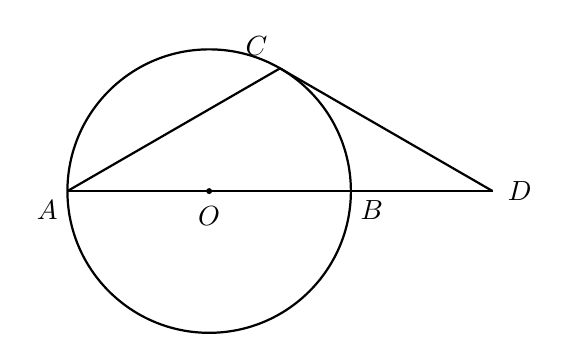
\begin{tikzpicture}[scale=0.9]
  % 半径 R=2，圆心 O=(2,0)；C 在圆心角 60° 处：C=(2+2cos60°, 2sin60°)=(3,1.732)
  % 切线 CD 与 x 轴交于 D=(6,0)
  \coordinate (A) at (0,0);
  \coordinate (O) at (2,0);
  \coordinate (B) at (4,0);
  \coordinate (C) at (3,1.732);
  \coordinate (D) at (6,0);
  \draw[thick] (O) circle (2);
  \draw[thick] (A) -- (D);
  \draw[thick] (A) -- (C);
  \draw[thick] (C) -- (D);
  \fill (O) circle (1.2pt) node[below=2pt] {$O$};
  \node[below left] at (A) {$A$};
  \node[below right] at (B) {$B$};
  \node[above left=1pt] at (C) {$C$};
  \node[right=2pt] at (D) {$D$};
\end{tikzpicture}
